% !TEX program = xelatex
\documentclass[UTF8,a4paper,12pt]{ctexart}

\usepackage{geometry}
\usepackage{amsmath,amssymb,bm}
\usepackage{booktabs,longtable,tabularx,array,multirow}
\usepackage{graphicx,float,subcaption}
\usepackage{enumitem}
\usepackage{hyperref}
\usepackage{xcolor}
\usepackage{caption}
\usepackage{siunitx}
\usepackage{titlesec}
\usepackage{fancyhdr}
\usepackage{lastpage}

\geometry{left=25mm,right=25mm,top=25mm,bottom=25mm}
\graphicspath{{figures/}}
\linespread{1.35}
\setlength{\parindent}{2em}
\setlist[itemize]{leftmargin=2.5em,itemsep=0.2em,topsep=0.2em}
\setlist[enumerate]{leftmargin=2.8em,itemsep=0.2em,topsep=0.2em}
\hypersetup{colorlinks=true,linkcolor=black,citecolor=black,urlcolor=black}
\captionsetup{font=small,labelfont=bf}
\pagestyle{fancy}
\fancyhf{}
\fancyhead[C]{纽约约租车调度决策}
\fancyfoot[C]{\thepage/\pageref{LastPage}}

\titleformat{\section}{\centering\heiti\zihao{4}}{\thesection}{0.8em}{}
\titleformat{\subsection}{\heiti\zihao{-4}}{\thesubsection}{0.6em}{}
\titleformat{\subsubsection}{\heiti\zihao{-4}}{\thesubsubsection}{0.6em}{}

\newcommand{\keywords}[1]{\par\vspace{0.5em}\noindent\textbf{关键词：}#1}
\newcommand{\R}{\mathbb{R}}

\begin{document}

\begin{center}
    {\heiti\zihao{3} 纽约约租车调度决策模型研究}\par
\end{center}

\begin{abstract}
本文围绕纽约市约租车平台在布鲁克林区域的需求预测、订单定价、车辆投放与基地选址问题，基于2019年1月黄车、绿车和FHV约租车记录，建立了从数据清洗、需求预测到运营决策的一体化模型。首先构造61个布鲁克林TLC区域的逐小时需求面板，并融合日历、天气和滞后需求特征，采用Poisson损失的梯度提升模型与历史均值基线加权融合，预测2019年2月1日各区域逐小时出发订单量；随后利用黄车和绿车数据训练出租车参考价格模型，并结合成本下界、最低利润率和拼车折扣，为115条FHV订单给出竞争性定价；在此基础上，构建以边际利润最大为原则的车辆整数分配模型，给出不同新增车辆规模下的中午12时车辆投放方案；最后建立加权$p$-中位选址模型，在布鲁克林61个区域中选出3个基地，使由基地到需求区的加权派车时间最小。

计算结果表明，需求预测模型在验证集上的MAE为1.9167，优于最优历史基线1.9820；FHV订单平均定价为15.96美元，平均成本口径利润率为56.18\%；当新增车辆数为100时，中午增量利润约为2183.85美元；当新增车辆数为200时，预测需求已由176辆车覆盖，剩余24辆可作为备用车辆。基地选址结果为Brooklyn Heights、Green-Wood Cemetery和Starrett City三个区域，相比按需求量直接选取前三个区域的方案，业务价值加权派车时间降低约28.00\%。模型具有较好的可解释性和可复现性，可为约租车平台在需求预测、价格制定和运力调度方面提供定量决策依据。
\keywords{约租车调度；需求预测；梯度提升；动态定价；车辆分配；$p$-中位模型}
\end{abstract}

\section{问题重述}
纽约市出租汽车与礼车委员会（TLC）监管的出行市场由传统出租车与约租车共同构成。黄车和绿车具有较完整的计价、里程、时长和上下车区域记录，而FHV约租车数据只给出订单时间、起终点区域和派车基地等字段。约租车平台希望在有限车辆资源下，利用历史出租车和约租车数据提高服务水平并扩大市场份额。题目要求解决以下四个相互衔接的问题：
\begin{enumerate}
    \item 结合黄车、绿车数据及必要外部数据，分析纽约市出租车在布鲁克林区域出发订单的分布规律，并预测2019年2月1日布鲁克林各区域逐小时订单量。
    \item 参考出租车计价规律，综合里程、时长、区域、时段和天气等因素，为附件3中FHV约租车订单设计价格方案。
    \item 在需求和价格模型基础上，针对2019年2月1日中午12时，给出布鲁克林各区域新增约租车的最优投放方案，并估计可能带来的收入和利润。
    \item 对特殊车型的基地出发式调度，规划3个布鲁克林区域作为基地位置，使派车时间、需求量和利润之间取得平衡。
\end{enumerate}
四个问题构成一个完整运营决策链：问题一给出区域--小时需求预测，问题二给出单笔订单价格与利润估计，问题三据此决定增配车辆的空间分布，问题四进一步为基地型车辆选择长期服务节点。

\section{问题分析与总体思路}
题目数据具有典型的多源、时空和业务链条特征。需求预测需要处理区域间强烈不均衡和小时周期性；订单定价需要在出租车参考价格、约租车竞争力和平台利润之间折中；车辆分配需要把车辆数这一整数资源投向边际收益最高的区域；基地选址则需要考虑从基地到需求区域的派车时间，并用需求和利润共同刻画服务价值。

本文采取“预测--定价--分配--选址”的递进式建模策略。首先将黄车和绿车订单清洗后聚合成布鲁克林61个区域、744个小时的完整面板；其次以该面板训练小时需求模型，得到2019年2月1日61个区域的逐小时需求；然后基于黄车和绿车的总费用训练参考价格模型，将参考价迁移到FHV订单，并加入成本和利润约束得到约租车价格；最后将中午12时需求、分区平均利润和平均服务时长作为车辆调度和基地选址的输入。该思路使每一问输出均服务于下一问，避免把预测、定价和调度割裂处理。总体流程如图\ref{fig:framework}所示。

\begin{figure}[H]
    \centering
    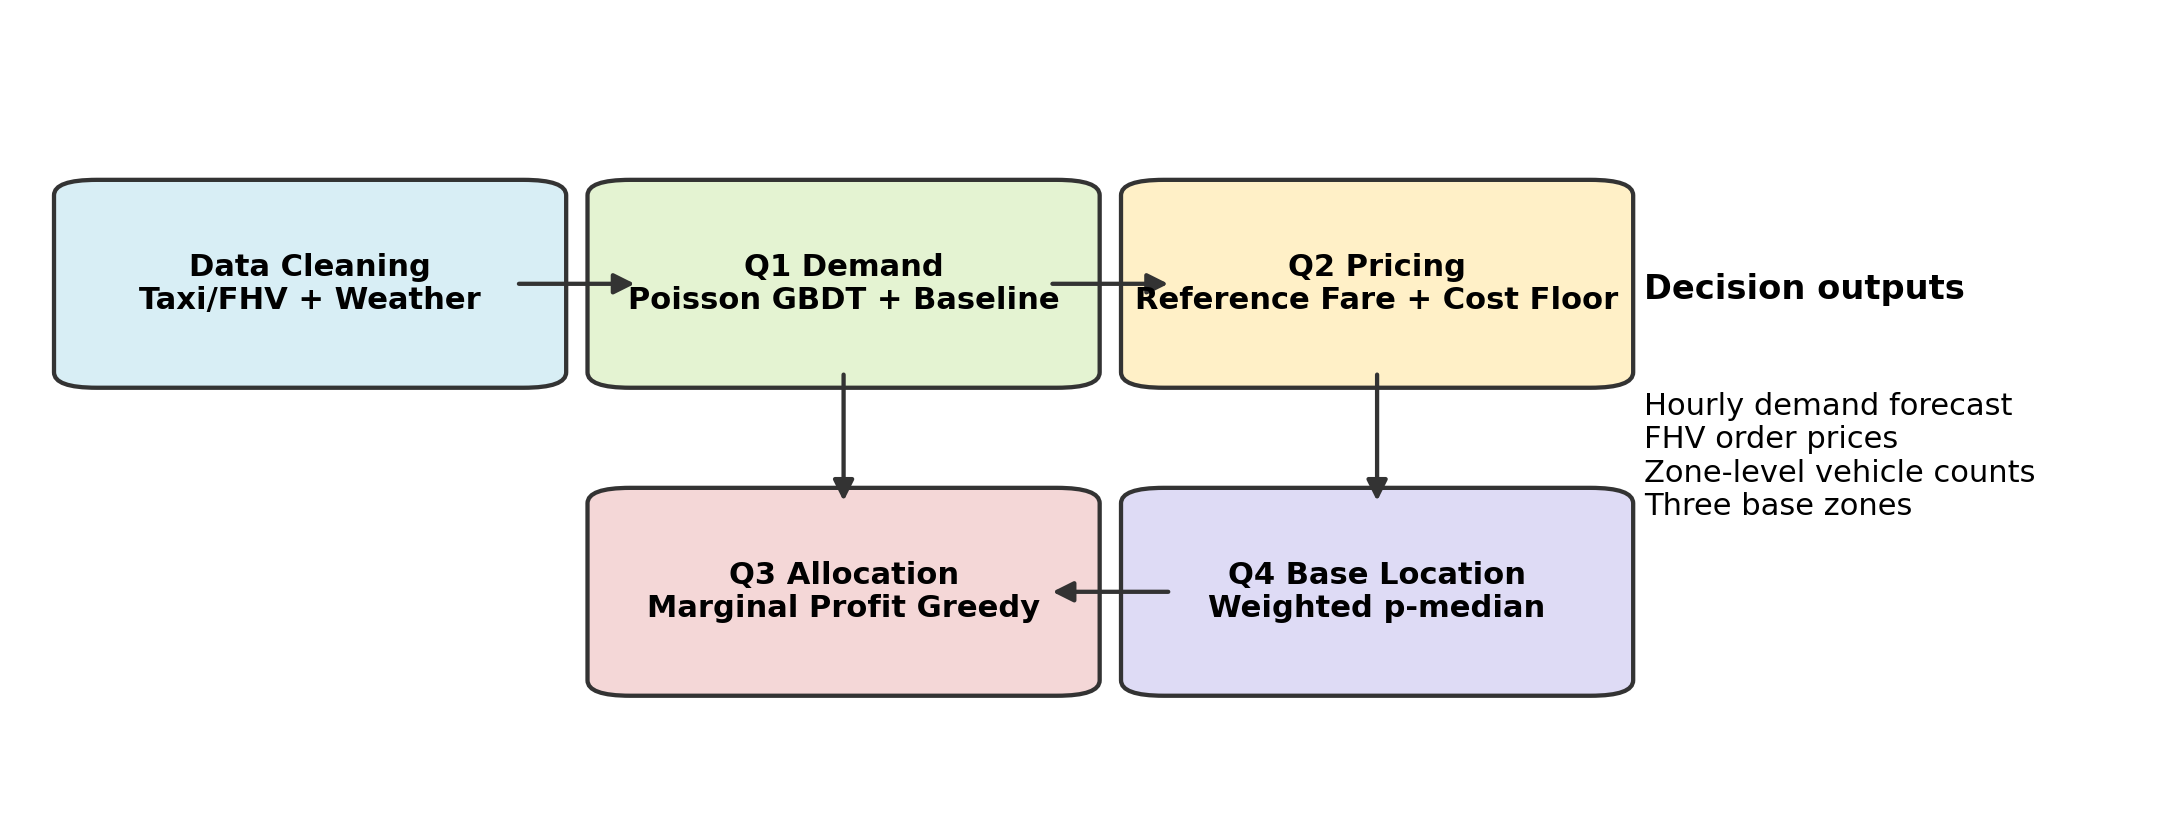
\includegraphics[width=0.92\textwidth]{model_framework.png}
    \caption{约租车调度决策建模流程}
    \label{fig:framework}
\end{figure}

从竞赛论文表达角度看，本文不把四个问题写成孤立小模型，而是把问题一的区域小时需求作为问题三和问题四的需求权重，把问题二的逐单利润转化为分区收益参数，使后续车辆投放和基地选址都具有明确的业务含义。这样既保留机器学习模型的预测能力，也保证优化结果可以解释为可执行的调度建议。

\section{模型假设}
\begin{enumerate}
    \item 2019年1月布鲁克林出租车出发订单可代表2019年2月1日的基本空间和小时分布规律；短期预测中不考虑平台促销、突发公共事件等未给出因素。
    \item 黄车与绿车订单的出发区域分布可作为FHV潜在可争取需求的主要参考。本文引入需求转化系数$\rho\in(0,1]$，令$\rho=1$作为基准上界情形；若平台目标份额较低，可按$\rho$对后续车辆需求和利润估计进行折减。FHV样本量较小导致的分区利润缺失用全局均值回填。
    \item 订单价格主要由距离、时长、起终点、时段、日历和天气因素决定；成本函数采用固定起步成本、里程成本和时间成本的线性形式。
    \item 车辆分配只研究2019年2月1日中午12时的静态增量投放，不考虑司机实时位置、订单取消、跨区后续再平衡和道路拥堵的动态反馈。
    \item 对缺少充足历史样本的OD对，使用TLC区域质心距离乘以绕行系数估计路程，并用历史平均速度估计时长。
    \item 基地选址结果为TLC区域层面的服务区选择，不等同于具体停车场或物业地址；落地时需在选中区域内进一步寻找合法停车和调度设施。
\end{enumerate}

\section{符号说明}
\begin{longtable}{p{0.22\textwidth}p{0.68\textwidth}}
\caption{主要符号说明}\label{tab:symbols}\\
\toprule
符号 & 含义 \\
\midrule
\endfirsthead
\toprule
符号 & 含义 \\
\midrule
\endhead
$i,z$ & TLC区域编号，本文主要研究布鲁克林61个区域 \\
$t$ & 小时时刻，训练期为2019年1月1日0时至1月31日23时 \\
$y_{i,t}$ & 区域$i$在小时$t$的出租车出发订单数 \\
$\bm{x}_{i,t}$ & 区域$i$在小时$t$的特征向量，包括时间、天气和滞后需求特征 \\
$\hat y_{i,t}$ & 区域$i$在小时$t$的预测出租车出发订单量 \\
$\rho$ & 出租车需求向FHV潜在可争取需求的转化系数，基准情形取$\rho=1$ \\
$d_k,T_k$ & 第$k$个订单的估计距离和服务时长 \\
$p^{ref}_k$ & 出租车参考价格模型给出的第$k$个订单参考价格 \\
$c_k,p_k,\pi_k$ & 第$k$个FHV订单的成本、最终定价和估计利润 \\
$D_i$ & 2019年2月1日中午12时区域$i$的FHV潜在可争取需求，$D_i=\rho\hat y_{i,12}$ \\
$\bar \pi_i,\bar T_i$ & 区域$i$的平均利润和平均服务时长 \\
$q_i$ & 区域$i$单辆车每小时服务能力，$q_i=60/\bar T_i$ \\
$n_i$ & 中午12时分配到区域$i$的新增车辆数 \\
$w_i$ & 基地选址中区域$i$的权重，$w_i=D_i\bar\pi_i$ \\
$B$ & 选中的3个基地区域集合 \\
$\tau_{j i}$ & 从基地区域$j$到需求区域$i$的派车时间 \\
\bottomrule
\end{longtable}
\section{数据预处理与探索性分析}

\subsection{数据来源与清洗}
本文使用附件1黄车数据、附件2绿车数据、附件3 FHV约租车数据、TLC区域对照表和出租车分区地图。黄车和绿车数据包含上下车时间、起终点区域、里程、费用等字段；FHV数据包含派车基地、上下车时间、起终点区域和是否拼车标记。为体现天气对需求和定价的影响，另引入布鲁克林经纬度附近的Open-Meteo历史小时天气数据，字段包括温度、降水、降雪指示、风速和能见度。

清洗规则包括：统一黄车、绿车和FHV的时间字段命名；计算服务时长；保留2019年1月内且起点为布鲁克林的订单；剔除非正里程、非正费用、异常长时长和明显错误时间记录。清洗结果如表\ref{tab:cleaning}所示。

\begin{table}[H]
\centering
\caption{原始数据清洗统计}
\label{tab:cleaning}
\begin{tabular}{lrrr}
\toprule
数据集 & 原始记录数 & 清洗后记录数 & 剔除记录数 \\
\midrule
黄车 & 85961 & 83354 & 2607 \\
绿车 & 196893 & 192749 & 4144 \\
FHV约租车 & 115 & 115 & 0 \\
\bottomrule
\end{tabular}
\end{table}

\subsection{区域--小时需求面板}
将清洗后的黄车和绿车订单按$(\text{区域},\text{小时})$聚合，得到完整的布鲁克林需求面板。布鲁克林共有61个TLC区域，2019年1月共有31天、744个小时，因此面板规模为$61\times744=45384$行。面板总订单量为276103，平均每个区域小时6.0837单，其中零需求区域小时为12123行。订单高峰小时为18时，总需求最高区域为Fort Greene，共22525单。

\begin{figure}[H]
    \centering
    \begin{subfigure}{0.48\textwidth}
        \centering
        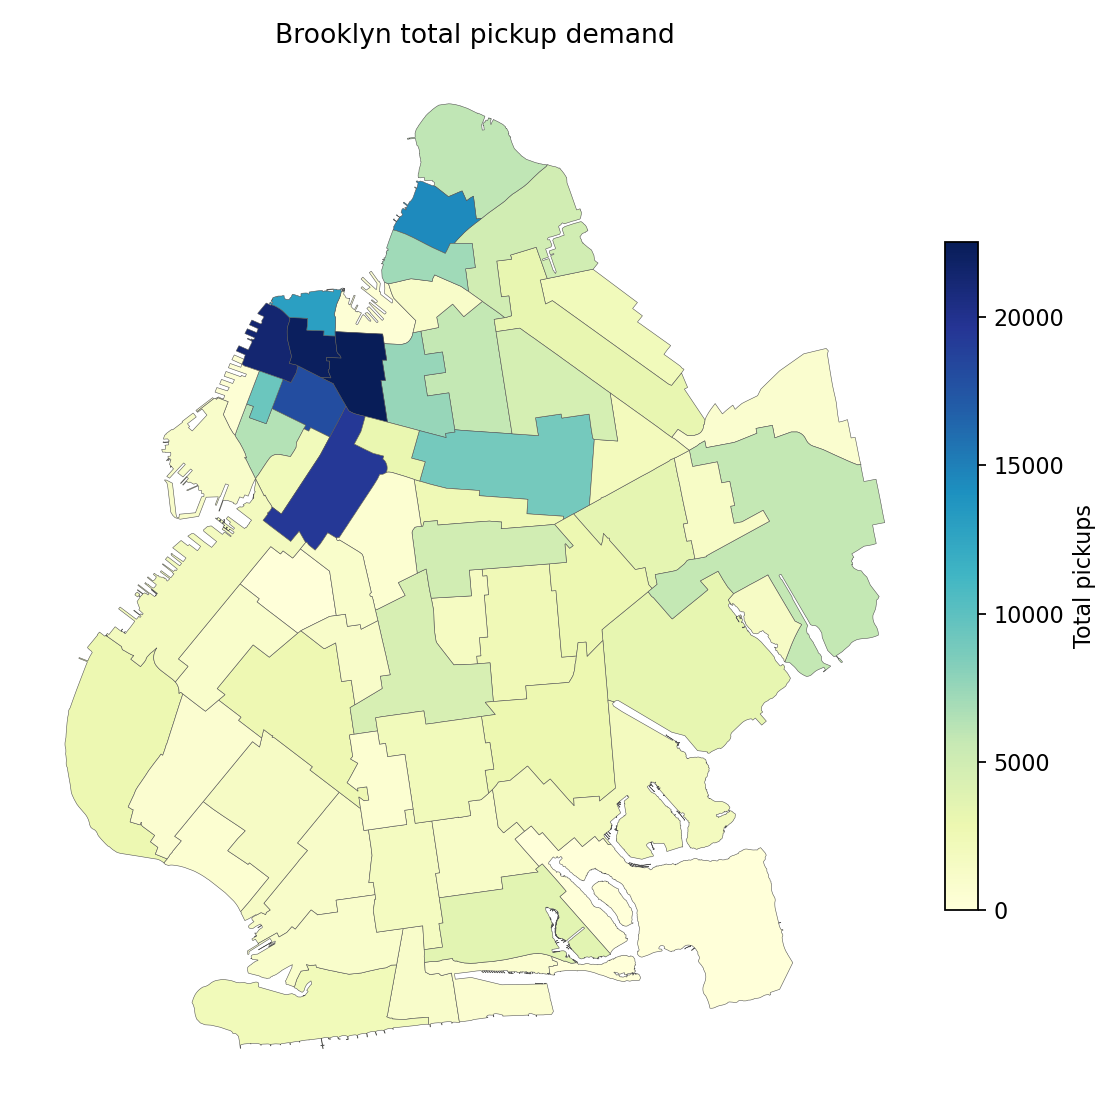
\includegraphics[width=\textwidth]{brooklyn_total_demand_map.png}
        \caption{布鲁克林总需求空间分布}
    \end{subfigure}
    \hfill
    \begin{subfigure}{0.48\textwidth}
        \centering
        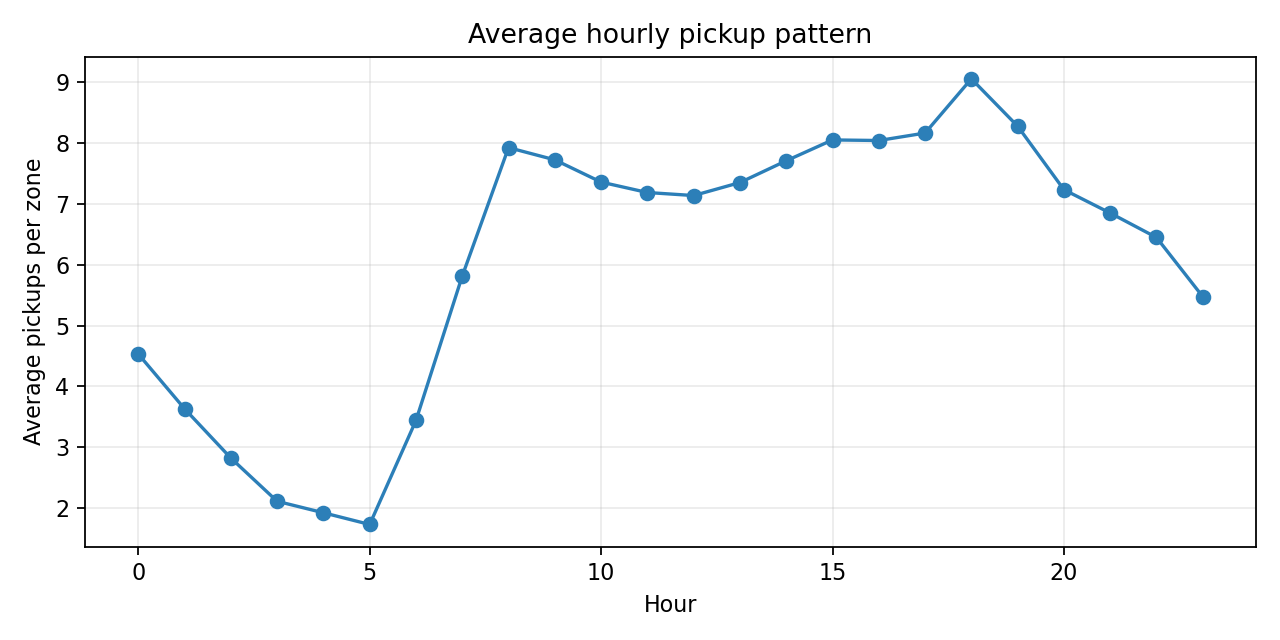
\includegraphics[width=\textwidth]{hourly_pattern.png}
        \caption{逐小时需求变化规律}
    \end{subfigure}
    \caption{布鲁克林出租车需求的空间与时间模式}
    \label{fig:eda}
\end{figure}

图\ref{fig:eda}显示，布鲁克林核心商业区与交通活跃区订单量明显更高，需求在早晚高峰和夜间出行时段具有较强周期性。进一步地，图\ref{fig:eda_more}给出高需求区域、工作日/周末模式和天气因素的关系。可以看出，订单集中于少数核心区域，且出行需求随星期类型和天气状态变化而波动。该特征说明，仅用全局平均值难以捕捉区域差异，需要在预测模型中引入区域编号、小时、星期、节假日、天气和历史滞后需求。

\begin{figure}[H]
    \centering
    \begin{subfigure}{0.48\textwidth}
        \centering
        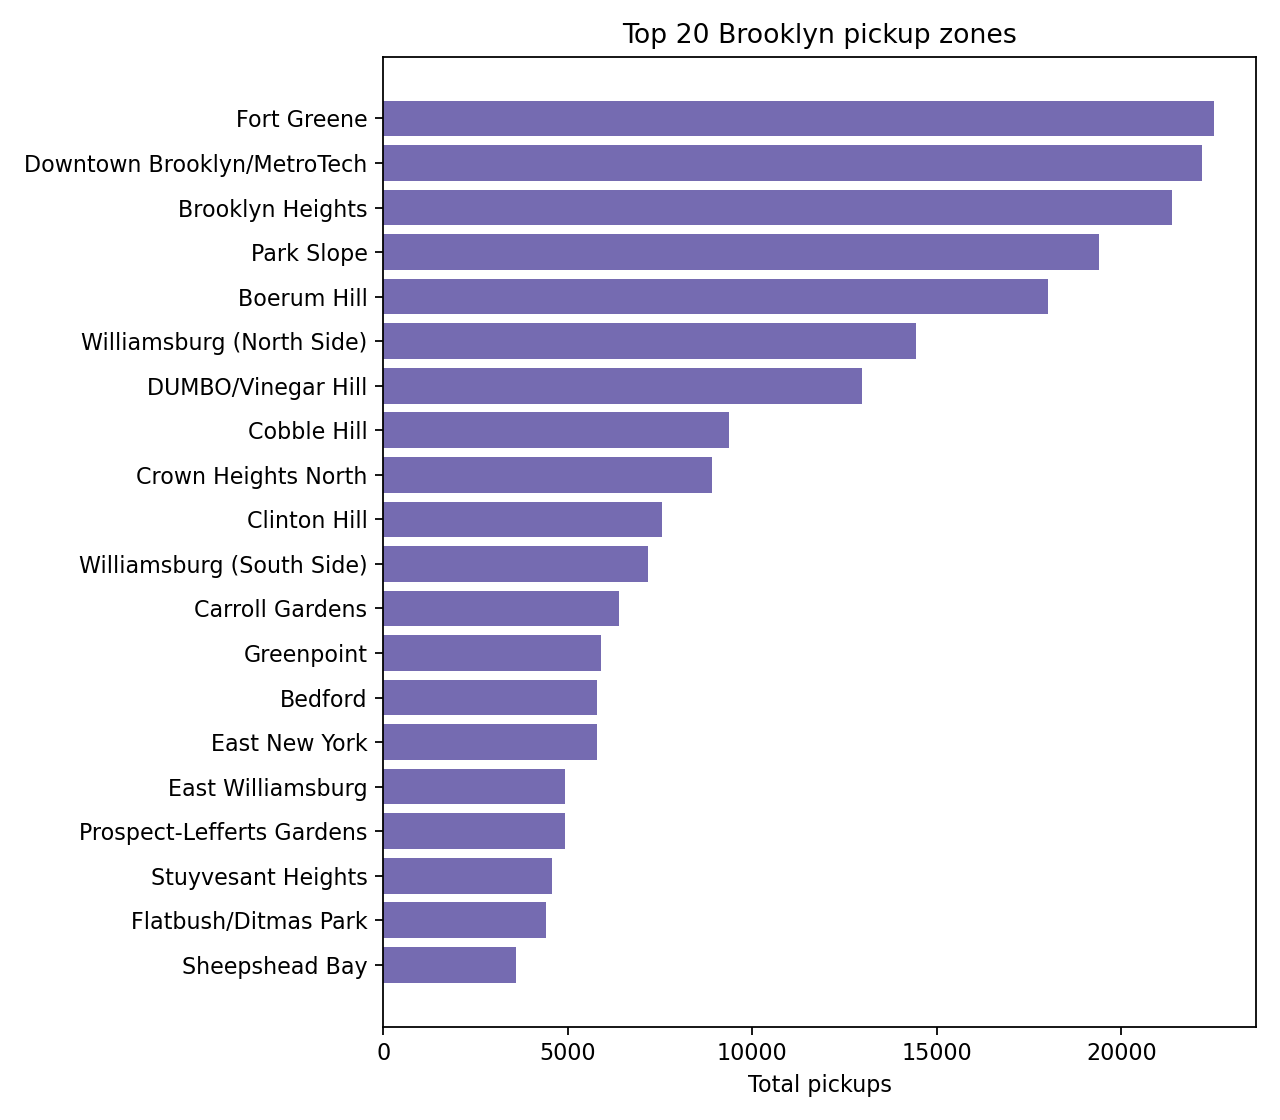
\includegraphics[width=\textwidth]{top20_zones.png}
        \caption{需求最高的20个TLC区域}
    \end{subfigure}
    \hfill
    \begin{subfigure}{0.48\textwidth}
        \centering
        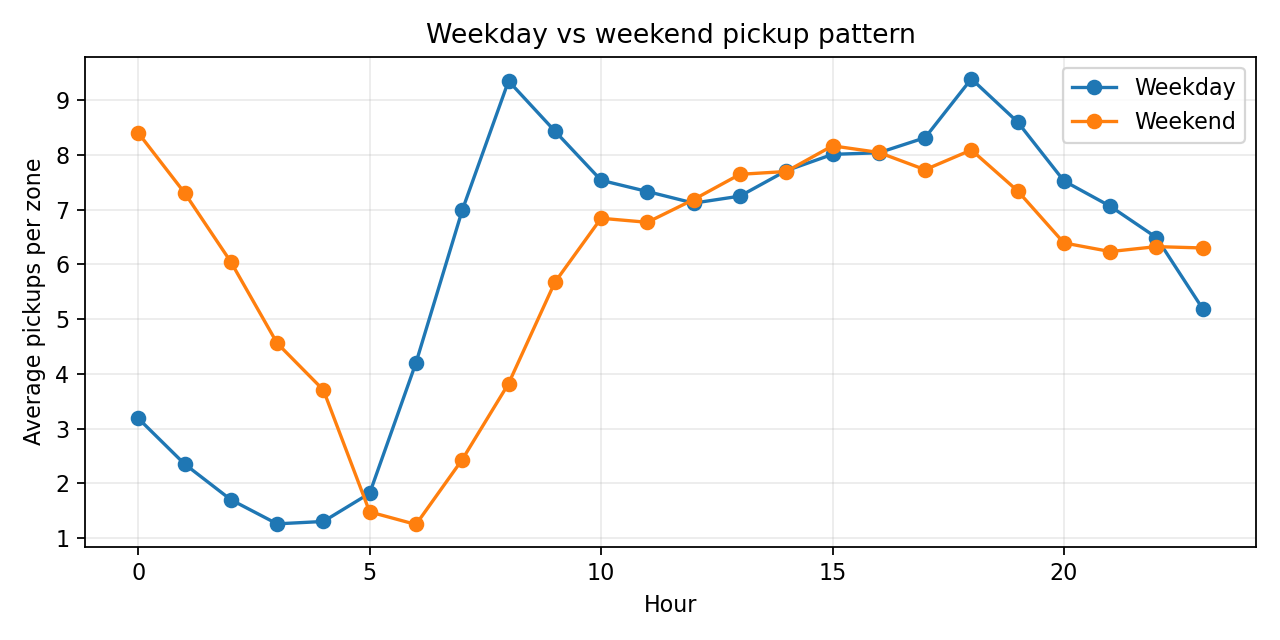
\includegraphics[width=\textwidth]{weekday_weekend_pattern.png}
        \caption{工作日与周末需求差异}
    \end{subfigure}
    \caption{布鲁克林需求的区域集中性与日历效应}
    \label{fig:eda_more}
\end{figure}

\begin{figure}[H]
    \centering
    
\includegraphics[width=0.76\textwidth]{weather_demand_relation.png}
    \caption{天气因素与布鲁克林出租车需求的关系}
    \label{fig:weather_demand}
\end{figure}

\section{问题一：订单需求预测模型}

\subsection{特征构造}
对每个区域$i$和小时$t$，目标变量为黄车与绿车出发订单数之和：
\begin{equation}
    y_{i,t}=y^{yellow}_{i,t}+y^{green}_{i,t}.
\end{equation}
特征向量$\bm{x}_{i,t}$由四类变量构成：区域编号；日历变量，包括小时、星期、是否周末、是否节假日、早晚高峰和夜间标记；天气变量，包括温度、降水、降雪指示、风速和能见度；滞后变量，包括$y_{i,t-24}$、$y_{i,t-168}$、过去24小时均值和过去168小时均值。小时变量同时采用正弦、余弦周期编码，以减少0时和23时在数值上的断裂。

\subsection{基线模型与融合预测}
为保证预测结果有可解释基准，本文构造三类历史均值基线：
\begin{align}
    \hat y^{(1)}_{i,t} &= \operatorname{mean}\{y_{i,s}: hour(s)=hour(t)\},\\
    \hat y^{(2)}_{i,t} &= \operatorname{mean}\{y_{i,s}: weekday(s)=weekday(t), hour(s)=hour(t)\},\\
    \hat y^{(3)}_{i,t} &= y_{i,t-168}.
\end{align}
主模型采用Poisson损失的直方图梯度提升回归模型$f_{\mathrm{GBDT}}(\bm{x})$。Poisson损失适用于非负计数型需求数据，可以避免线性模型对高峰时段和低需求区域的拟合能力不足。训练集为2019年1月1日至1月24日，验证集为1月25日至1月31日。

为了兼顾机器学习模型的非线性拟合能力和历史基线的稳定性，最终预测采用凸组合：
\begin{equation}
    \hat y_{i,t}=\alpha f_{\mathrm{GBDT}}(\bm{x}_{i,t})+(1-\alpha)\hat y^{base}_{i,t},
\end{equation}
其中$\hat y^{base}$取验证集表现最好的“区域--星期--小时均值”基线，$\alpha$通过验证集网格搜索确定。实验得到$\alpha=0.4$，即主模型权重为0.4，基线权重为0.6。

\subsection{预测结果}
模型评估结果如表\ref{tab:q1_metrics}所示。融合模型MAE为1.9167，低于最佳历史基线1.9820，也优于Poisson GBDT单模型的MAE 2.1041，说明加入天气、滞后需求和非线性模型后，对区域小时需求的平均绝对误差有所降低。SMAPE在大量零需求或低需求区域中会放大小分母误差，且融合模型的主要用途是后续车辆调度中的订单量估计，因此本文主要采用MAE和RMSE评价预测精度。

\begin{table}[H]
\centering
\caption{需求预测模型验证结果}
\label{tab:q1_metrics}
\begin{tabular}{lccc}
\toprule
模型 & MAE & RMSE & SMAPE \\
\midrule
区域--星期--小时均值 & 1.9820 & 3.7733 & 0.6587 \\
上周同小时 & 2.3919 & 4.6179 & 0.6354 \\
区域--小时均值 & 2.4177 & 5.2138 & 0.8414 \\
GBDT与基线融合 & 1.9167 & 3.6289 & 0.8500 \\
\bottomrule
\end{tabular}
\end{table}

\begin{figure}[H]
    \centering
    
\includegraphics[width=0.82\textwidth]{model_validation_compare.png}
    \caption{验证集布鲁克林总需求真实值与模型预测值对比}
    \label{fig:validation}
\end{figure}

将模型用于2019年2月1日预测，得到61个区域、24个小时共1464条预测记录，全天总预测出租车出发需求为9785.92单。中午12时全布鲁克林预测需求为427.69单。本文在基准情形下取$\rho=1$，将其视为FHV平台可争取需求的上界输入；当实际市场份额低于该上界时，可用$D_i=\rho\hat y_{i,12}$对车辆规模和利润进行比例修正。

\section{问题二：约租车订单定价模型}

\subsection{出租车参考价格模型}
FHV数据缺少里程和费用字段，不能直接用FHV历史价格建模。本文先利用黄车和绿车数据学习出租车参考价格，再将该参考价格迁移到FHV订单。对订单$k$，参考价格模型为
\begin{equation}
    p^{ref}_k=f(d_k,T_k,PU_k,DO_k,hour_k,weekday_k,weather_k),
\end{equation}
其中$d_k$和$T_k$分别表示距离和时长，$PU_k,DO_k$为起终点区域。模型同样采用直方图梯度提升回归，损失函数为平方误差；从出租车样本中按随机种子20260619抽取不超过120000条记录，并按8:2划分训练集和验证集。核心参数设为learning rate 0.06、最大迭代180、最大叶节点31和$L_2$正则0.05。

对FHV订单，距离字段由历史出租车OD对估计：若其OD对在黄车和绿车历史数据中有不少于3条样本，则取该OD对历史中位距离；否则使用区域质心距离乘以1.3作为回退估计。由于附件3给出了上下车时间，本文在样本回放定价中使用观测服务时长；若用于事前报价，可用同一OD中位时长替代观测时长。115条FHV订单中，109条使用历史中位距离估计，6条使用质心距离回退。

\subsection{成本约束与定价公式}
约租车平台既要保持相对出租车的价格竞争力，又不能低于成本和最低利润要求。本文设定线性成本函数：
\begin{equation}
    c_k=2.75+1.15d_k+0.18T_k,
\end{equation}
其中2.75美元为基础成本，1.15美元/英里为里程成本，0.18美元/分钟为时间成本。设最低利润率$r_{\min}=15\%$，相对出租车参考价的折扣率$\delta=8\%$，先得到基础价格
\begin{equation}
    p^0_k=\max\{c_k(1+r_{\min}),\; p^{ref}_k(1-\delta)\}.
\end{equation}
若订单为拼车订单，则在基础价格上给予拼车折扣因子$\gamma=0.90$，但折扣后仍不能低于最低利润底线：
\begin{equation}
    p_k=\begin{cases}
    \max\{\gamma p^0_k,\;c_k(1+r_{\min})\}, & \text{拼车订单},\\
    p^0_k, & \text{非拼车订单}.
    \end{cases}
\end{equation}
该规则兼顾价格优势、拼车激励和利润底线，避免因拼车折扣造成低于成本加最低利润的报价。

\subsection{定价结果}
表\ref{tab:q2_summary}给出定价模型汇总结果。出租车参考价模型在验证集上的MAE为1.9077美元，说明其能够较好刻画出租车总费用规律。对115条FHV订单，平均出租车参考价为17.55美元，平均FHV定价为15.96美元，平均估计成本为10.12美元。本文定义逐单成本口径利润率为$r_k=(p_k-c_k)/c_k$，其样本平均值为56.18\%；若按价格口径$(p_k-c_k)/p_k$计算，平均值约为35.66\%。平均FHV价格低于出租车参考价，体现了约租车的竞争性；同时由于短途订单成本较低，整体仍保持较高利润空间。

\begin{table}[H]
\centering
\caption{FHV订单定价模型结果}
\label{tab:q2_summary}
\begin{tabular}{lr}
\toprule
指标 & 数值 \\
\midrule
出租车参考价训练样本数 & 120000 \\
参考价模型MAE/美元 & 1.9077 \\
FHV订单数 & 115 \\
平均出租车参考价/美元 & 17.55 \\
平均FHV定价/美元 & 15.96 \\
平均估计成本/美元 & 10.12 \\
平均估计利润率（成本口径） & 56.18\% \\
\bottomrule
\end{tabular}
\end{table}
\begin{figure}[H]
    \centering
    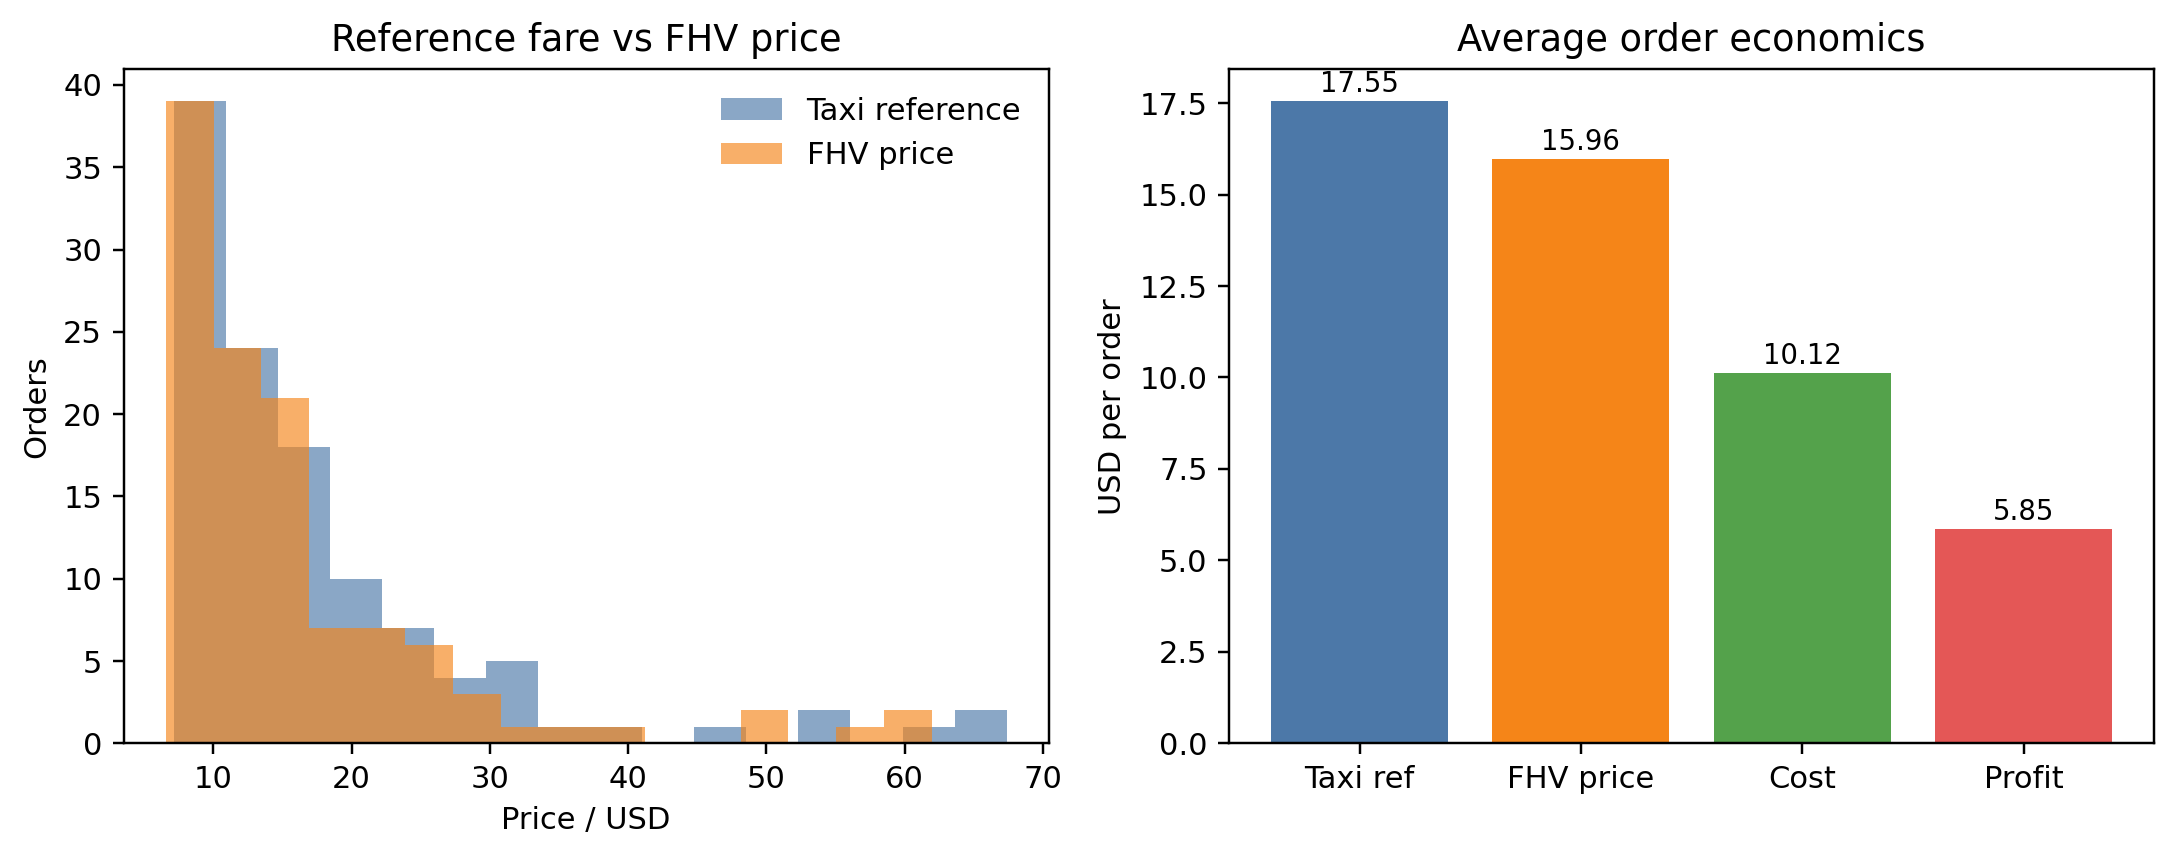
\includegraphics[width=0.82\textwidth]{pricing_economics.png}
    \caption{FHV定价结果与订单经济性对比}
    \label{fig:pricing_economics}
\end{figure}

图\ref{fig:pricing_economics}表明，FHV定价整体低于出租车参考价，但仍高于估计成本，说明竞争折扣和成本底线同时起作用。该图也解释了为什么后续车辆分配不能只看需求量，还需要结合分区利润。
\section{问题三：新增车辆区域分配模型}

\subsection{边际利润分配策略}
问题三要求在新增车辆数给定时，确定2019年2月1日中午12时布鲁克林各区域投放车辆数。令$D_i=\rho\hat y_{i,12}$为区域$i$中午FHV潜在可争取需求，$\bar\pi_i$为问题二定价结果在区域$i$的平均利润，$\bar T_i$为平均服务时长，则单辆车在一小时内服务能力为
\begin{equation}
    q_i=\frac{60}{\bar T_i}.
\end{equation}

设当前区域$i$已服务需求为$s_i$。每新增一辆车到区域$i$可带来的边际服务量为
\begin{equation}
    m_i=\min\{q_i,\,D_i-s_i\}_{+},
\end{equation}
相应边际利润为$m_i\bar\pi_i$。本文采用贪心整数分配：每次把一辆车分配给$m_i\bar\pi_i$最大的区域，直到车辆用完或所有区域需求均被覆盖。若需求已饱和而车辆仍有剩余，则剩余车辆记为闲置或备用车辆，不再强行分配到某一区域。由于$q_i$只按车上服务时长计算，未显式扣除接驾、等待和空驶时间，因此该分配结果可视为静态单小时理想上界；实际运营中可进一步用有效服务系数对$q_i$折减。

\subsection{分配结果}
基准情形$\rho=1$下，中午12时全布鲁克林潜在可争取需求上界为427.69单。表\ref{tab:q3_summary}列出不同车辆规模下的服务量和收益。新增50辆和100辆车时，所有车辆均被分配；新增200辆时，仅需176辆即可覆盖全部预测需求，剩余24辆作为备用，继续增加至250辆不再带来额外收益。

\begin{table}[H]
\centering
\caption{中午12时新增车辆分配收益}
\label{tab:q3_summary}
\begin{tabular}{rrrrrr}
\toprule
新增车辆数 & 实际分配车辆 & 闲置车辆 & 服务需求 & 增量收入/美元 & 增量利润/美元 \\
\midrule
50 & 50 & 0 & 190.79 & 3248.27 & 1283.51 \\
100 & 100 & 0 & 294.92 & 5625.41 & 2183.85 \\
200 & 176 & 24 & 427.69 & 7645.05 & 2867.93 \\
\bottomrule
\end{tabular}
\end{table}

\begin{figure}[H]
    \centering
    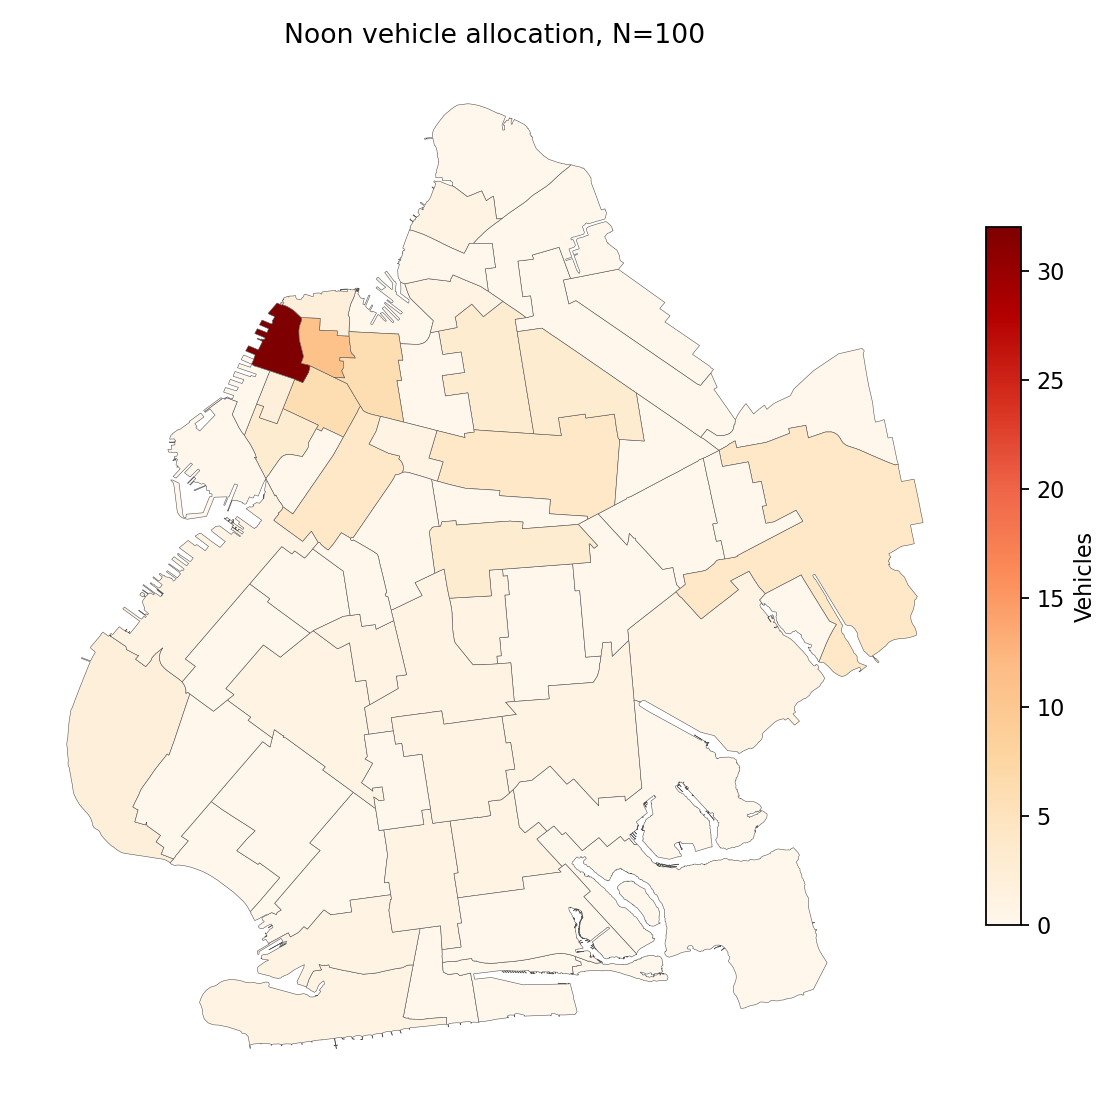
\includegraphics[width=0.72\textwidth]{vehicle_allocation_map.png}
    \caption{$N=100$时布鲁克林新增车辆空间分配}
    \label{fig:vehicle_allocation}
\end{figure}

\begin{figure}[H]
    \centering
    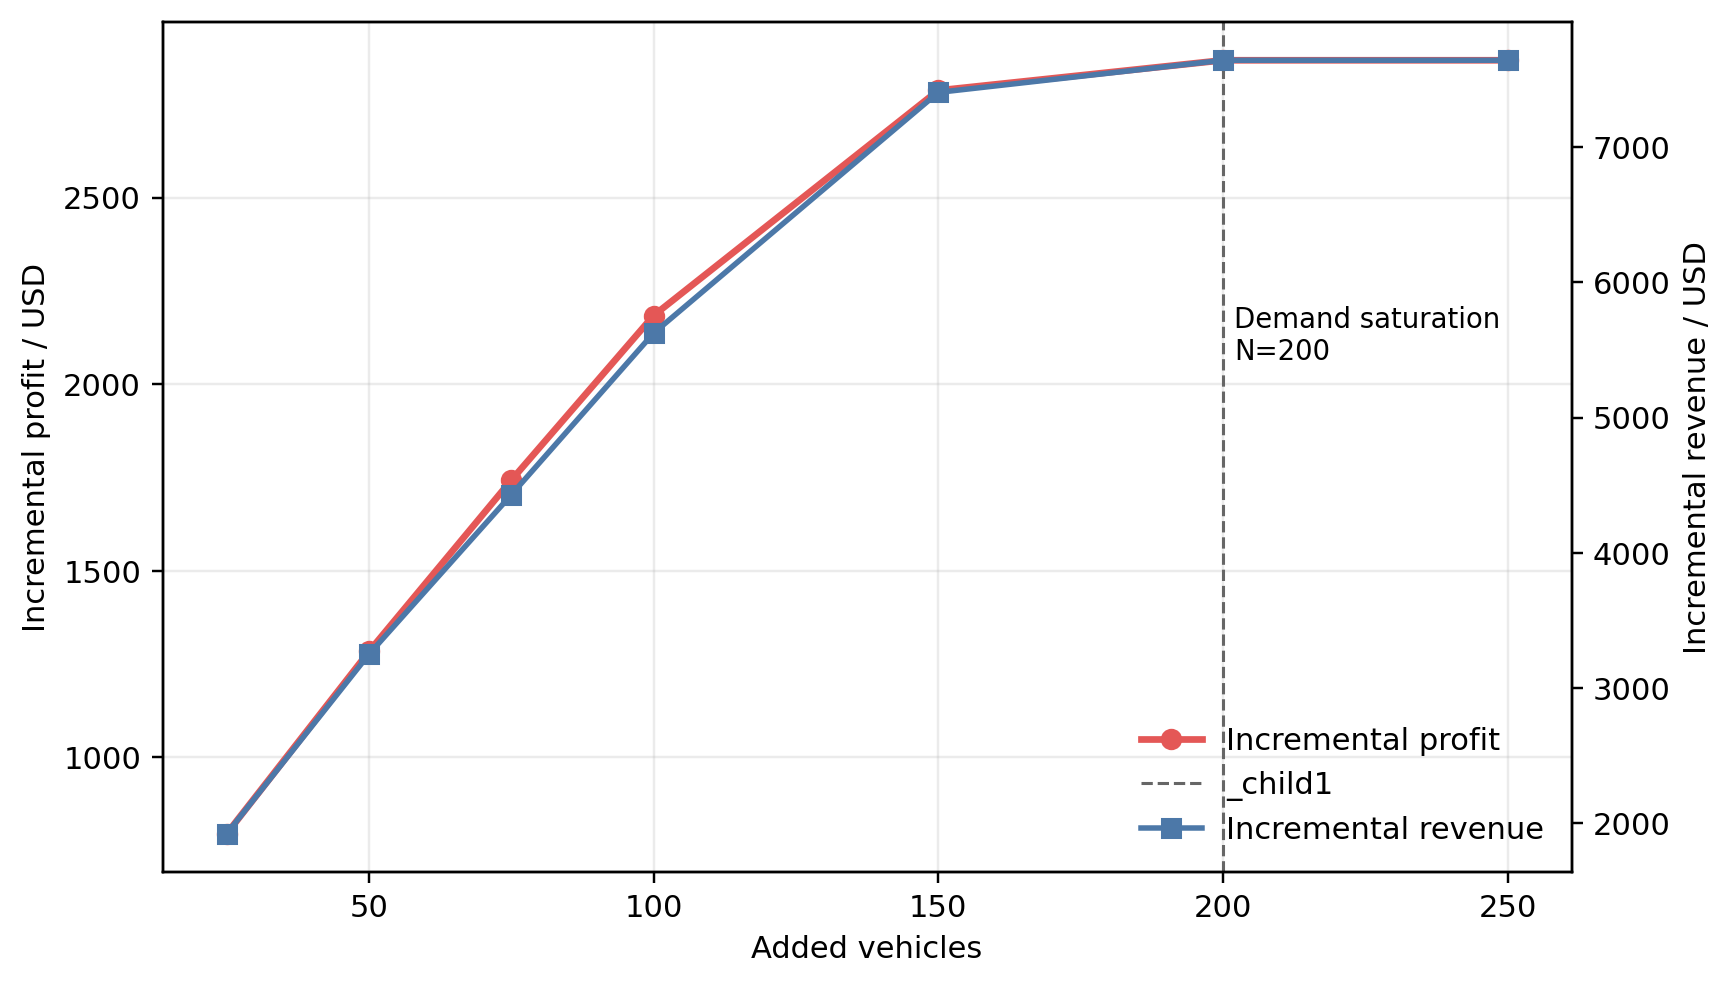
\includegraphics[width=0.78\textwidth]{vehicle_profit_sensitivity.png}
    \caption{新增车辆规模对中午增量收益的影响}
    \label{fig:vehicle_profit_sensitivity}
\end{figure}

图\ref{fig:vehicle_profit_sensitivity}显示，车辆规模从25辆增加到150辆时，增量利润增长较快；当车辆数接近200辆后，预测需求基本被覆盖，继续增加车辆只会形成备用运力，边际收益趋于零。
从图\ref{fig:vehicle_allocation}可以看出，车辆主要投向Downtown Brooklyn/MetroTech、Brooklyn Heights、Boerum Hill、Fort Greene等需求密集且利润较高的区域。该结果与需求热力图基本一致，但并非完全按需求排序，而是同时考虑服务时长和利润。

\section{问题四：三基地选址模型}

\subsection{加权$p$-中位模型}
特殊车型从基地出发前往上客区域，因此基地选址应最小化“基地到需求区”的派车时间。令$B$为选中的基地区域集合，$|B|=3$；令$\tau_{ji}$为从基地区域$j$到需求区域$i$的估计派车时间；令$w_i=D_i\bar\pi_i$表示区域$i$的业务价值权重。选址模型为
\begin{equation}
    \min_{B\subseteq \mathcal{Z},\,|B|=3}
    \sum_{i\in\mathcal{Z}} w_i \min_{j\in B}\tau_{ji}.
    \label{eq:pmedian}
\end{equation}

其中$\mathcal{Z}$为布鲁克林61个TLC区域集合。由于候选组合数为$\binom{61}{3}=35990$，规模较小，本文采用穷举法求全局最优，并与三类基准方案比较：按需求量最高的3个区域选址、随机选3个区域、按地理KMeans聚类选3个区域。

\subsection{选址结果}
表\ref{tab:q4_summary}显示，最优$p$-中位方案选择Brooklyn Heights、Green-Wood Cemetery和Starrett City三个区域作为基地。目标函数数值为业务价值权重与派车时间的乘积和，并非直接的美元成本；为表述简洁，下文称其为“业务价值加权派车时间”。最优方案的加权派车时间为26190.96，相比按需求量前三区域（Brooklyn Heights、Downtown Brooklyn/MetroTech、Fort Greene）选址的36375.70，降低约28.00\%。这说明仅追求需求高地会导致东南部和西南部区域服务距离过长，而$p$-中位模型能在高需求中心和边缘覆盖之间取得更均衡的布局。

\begin{table}[H]
\centering
\caption{三基地选址方案对比}
\label{tab:q4_summary}
\begin{tabularx}{\textwidth}{lXrr}
\toprule
方案 & 基地区域 & 业务价值加权派车时间 & 相对需求Top3改善 \\
\midrule
最优$p$-中位 & 33 Brooklyn Heights；111 Green-Wood Cemetery；222 Starrett City & 26190.96 & 27.999\% \\
需求Top3 & 33 Brooklyn Heights；65 Downtown Brooklyn/MetroTech；97 Fort Greene & 36375.70 & 0 \\
地理KMeans & 35 Brownsville；97 Fort Greene；178 Ocean Parkway South & 31460.55 & 13.512\% \\
随机方案（固定种子示例） & 21 Bensonhurst East；150 Manhattan Beach；228 Sunset Park West & 58924.00 & -61.987\% \\
\bottomrule
\end{tabularx}
\end{table}

\begin{figure}[H]
    \centering
    
\includegraphics[width=0.72\textwidth]{base_location_map.png}
    \caption{最优三基地方案及服务区域分配}
    \label{fig:base_location}
\end{figure}

需要说明的是，Green-Wood Cemetery和Starrett City等名称代表TLC分区，不意味着基地必须设在墓园或住宅内部。实际落地时，应在对应TLC区域内进一步筛选可停车、可充电、可调度的合法物业或路外停车设施。

\section{灵敏度分析与模型评价}

\subsection{灵敏度分析}
本文从定价参数、车辆规模和需求转化系数三方面做灵敏度分析。定价方面，将最低利润率取0.10、0.15、0.20，折扣率取0.05、0.08、0.12，得到9组情形。结果表明，折扣率从5\%增至12\%时，平均FHV价格由约16.49美元降至15.27美元，平均成本口径利润率由61.27\%降至49.39\%；在当前样本下，最低利润率变化对结果影响较小，说明多数订单由出租车参考价折扣约束决定，而非成本底线决定。

\begin{table}[H]
\centering
\caption{关键参数灵敏度结果}
\label{tab:sensitivity}
\begin{tabular}{lrr}
\toprule
情形 & 平均FHV价格/美元 & 平均利润率或增量利润 \\
\midrule
折扣率5\% & 16.49 & 61.27\% \\
折扣率8\% & 15.96 & 56.18\% \\
折扣率12\% & 15.27 & 49.39\% \\
车辆数$N=25$ & -- & 795.04美元 \\
车辆数$N=100$ & -- & 2183.85美元 \\
车辆数$N=200$ & -- & 2867.93美元 \\
车辆数$N=250$ & -- & 2867.93美元 \\
\bottomrule
\end{tabular}
\end{table}

车辆规模方面，分别考察$N=25,50,75,100,150,200,250$。增量利润从$N=25$的795.04美元增加到$N=150$的2787.11美元；当$N=200$时达到2867.93美元并覆盖全部中午预测需求，继续增加到$N=250$时利润不再增长。这说明车辆投放存在明显边际收益递减，平台不宜只追求车辆数量扩张，而应结合需求峰值和服务能力确定备用规模。需求转化系数方面，若$\rho<1$，则各区需求$D_i$整体下降，在车辆尚未达到需求饱和前，服务量和增量利润近似随$\rho$同比例缩小；在车辆充足情形下，饱和所需车辆数也相应下降。

\subsection{模型优点}
\begin{itemize}
    \item 模型链条完整：需求预测、订单定价、车辆投放和基地选址逐级衔接，符合平台实际决策流程。
    \item 预测模型兼顾非线性与稳定性：Poisson GBDT能够捕捉复杂特征，历史基线融合避免小样本区域过拟合。
    \item 定价模型可解释：成本底线、最低利润率、竞争折扣和拼车折扣均具有明确业务含义，且拼车折扣后仍保留利润下界。
    \item 调度模型保持整数可行性：车辆逐辆分配，结果可直接转化为区域车辆数，并允许需求饱和后的备用车辆。
    \item 选址模型可求全局最优：在61个区域中穷举三基地组合，避免启发式算法陷入局部最优。
\end{itemize}

\subsection{模型不足与改进方向}
\begin{itemize}
    \item 需求预测只基于一个月数据，对跨月季节性、重大活动和突发天气的泛化能力有限。
    \item FHV样本仅115条，定价实质上是出租车参考价向FHV迁移，未来应引入更大规模FHV实际成交价。
    \item OD时间估计部分依赖区域质心距离，未使用真实道路网络和实时拥堵数据，可能低估绕行和过桥时间。
    \item 车辆分配模型为单小时静态上界模型，未考虑接驾等待、车辆完成订单后的空间再分布和司机接单行为。
    \item 基地选址只到TLC区域层级，实际建设还需考虑停车、充电、租金、法规和司机换班便利性。
\end{itemize}

\section{结论}
本文基于纽约市2019年1月出租车和FHV记录，构建了面向约租车平台的调度决策模型。首先，构造布鲁克林61个区域的小时需求面板，并利用Poisson梯度提升模型与历史基线融合预测2019年2月1日需求，验证集MAE为1.9167。其次，利用黄车和绿车费用数据建立出租车参考价模型，并在成本和竞争约束下为115条FHV订单定价，平均价格为15.96美元，平均成本口径利润率为56.18\%。再次，以出租车出发需求作为FHV潜在可争取需求上界，结合中午需求、分区利润和服务能力进行车辆整数分配，$N=100$时预计增量利润2183.85美元，$N=200$时176辆车即可覆盖全部预测需求。最后，建立加权$p$-中位基地选址模型，选出Brooklyn Heights、Green-Wood Cemetery和Starrett City三个基地分区，相比按需求量直接选址的方案，业务价值加权派车时间降低约28.00\%。

整体来看，本文模型能够把历史数据转化为可执行的价格、车辆和基地决策方案。若未来获得更长时间跨度、更完整FHV价格、更精细道路网络和实时车辆状态数据，可进一步扩展为动态滚动调度模型，提高对真实平台运营的适应性。

\begin{thebibliography}{9}
\bibitem{tlcdata} New York City Taxi and Limousine Commission. TLC Trip Record Data and Data Dictionaries.
\bibitem{openmeteo} Open-Meteo. Historical Weather API documentation.
\bibitem{sklearn} Scikit-learn Developers. HistGradientBoostingRegressor documentation.
\bibitem{hakimi} Hakimi S L. Optimum locations of switching centers and the absolute centers and medians of a graph. Operations Research, 1964.
\end{thebibliography}

\end{document}
